\chapter{Resultados en las ligas}
\label{cap:resligas}

\section{Partidos frente al mercado (R1)}

El núcleo, sin tiros, alcanza un RPS de 0,1995 en 18.700 partidos de las cinco grandes ligas entre 2016 y 2026, frente a 0,1941 de Bet365. En el Brasileirão, 0,2065 frente a 0,1999. En Chile, donde no hay cuotas en el espejo, se compara con las frecuencias históricas: 0,2241 frente a 0,2306. Para tener una escala, en el \emph{Soccer Prediction Challenge} de 2017 los cuatro primeros quedaron separados por 0,003 de RPS~\cite{berrar2019}. Las diferencias entre buenos modelos de goles son chicas; las diferencias con el mercado, en cambio, son estables.

\section{Crear y convertir (R13)}

Fuera de muestra (desde 2016; Chile desde 2020), el modelo de dos latentes mejora la log-verosimilitud del marcador frente al núcleo en el conjunto de las ligas (figura~\ref{fig:dos}, izquierda). La ganancia es clara en la Premier ($+0{,}0093\pm0{,}0023$ nats por partido; RPS 0,1982 frente a 0,1999 del núcleo y 0,1936 de Bet365), en Chile ($+0{,}0042\pm0{,}0017$), en la Ligue 1 ($+0{,}0052\pm0{,}0024$), en la Championship ($+0{,}0075\pm0{,}0015$, $z=4{,}9$) y, en menor medida, en Argentina ($+0{,}0035\pm0{,}0019$). En el Brasileirão, la Serie A, LaLiga y la Bundesliga la diferencia no alcanza dos errores estándar, y en ninguna liga empeora de forma significativa. Combinando las nueve ligas por la inversa de la varianza, la ganancia es $+0{,}0036\pm0{,}0006$ nats por partido ($z=5{,}9$). En las siete primeras la heterogeneidad era moderada ($Q=15{,}8$ con 6 grados de libertad), con la Premier como la liga que más gana.

\begin{figure}[h]
\centering
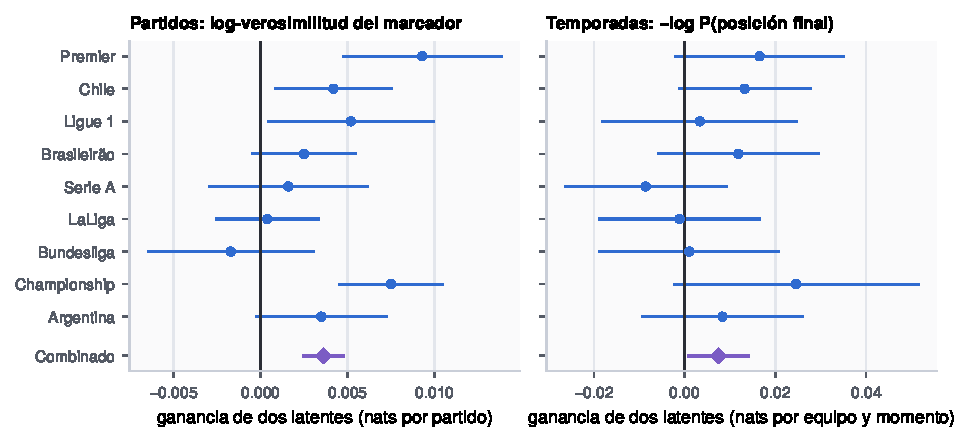
\includegraphics[width=\textwidth]{dos_latentes}
\caption{Ganancia del modelo de dos latentes frente al núcleo, fuera de muestra, con barras de dos errores estándar. Izquierda: log-verosimilitud del marcador por partido. Derecha: log score de la posición final, por equipo y momento de la temporada (pretemporada, 25, 50 y 75\,\%). El rombo es el promedio ponderado por la inversa de la varianza (izquierda) y el promedio agrupado de todas las temporadas (derecha).}
\label{fig:dos}
\end{figure}

Lo que agrega el modelo es no confundir una racha de conversión con fuerza. Un equipo que convierte la mitad de sus tiros al arco baja, porque el modelo espera que esa conversión revierta; uno al que le convierten casi cada tiro en contra sube.

\section{La tabla final (R16)}

Lo que muestra el sitio son posiciones finales, y ahí la pregunta es otra. El backtest pareado de la posición final real ($-\log P$), en pretemporada y al 25, 50 y 75\,\% de cada temporada, con hiperparámetros fuera de muestra, da $+0{,}0075\pm0{,}0034$ nats por equipo y momento a favor de dos latentes en 84 temporadas de nueve ligas (figura~\ref{fig:dos}, derecha). Por liga ninguna muestra evidencia de que pierda. En las siete ligas originales (64 temporadas) la ganancia estaba en la segunda mitad de la temporada ($+0{,}008$ al 50\,\% y $+0{,}012$ al 75\,\%) y era nula en pretemporada, como se espera: ahí manda la regresión a la media entre temporadas, no la conversión. Con la Championship y Argentina, la ganancia por momento queda en $+0{,}010$ en pretemporada, $+0{,}004$ al 25\,\%, $+0{,}007$ al 50\,\% y $+0{,}009$ al 75\,\%; la de pretemporada viene de esas dos ligas. En los mismos 17.910 partidos del top 5 con cuotas, el RPS de dos latentes es 0,1990 (núcleo 0,1995, Bet365 0,1941); en la Premier, 0,1977 frente a 0,1936.

\section{Incertidumbre calibrada (R2)}

\begin{figure}[h]
\centering
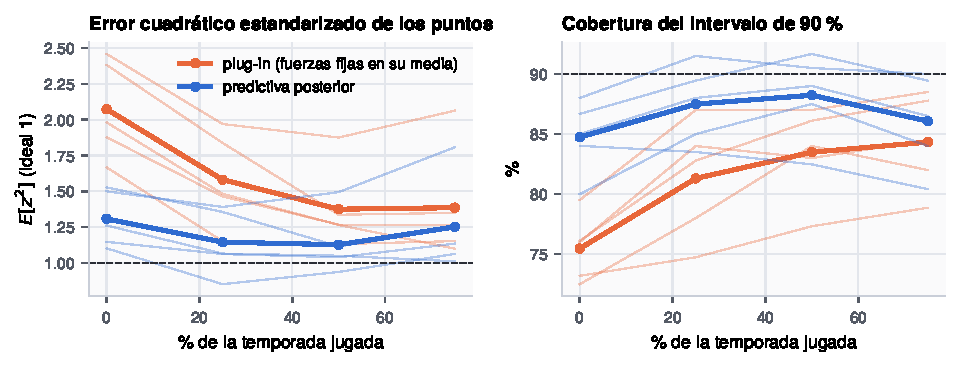
\includegraphics[width=\textwidth]{varianza}
\caption{Calibración de los puntos finales en las cinco grandes ligas, 2016-2025, según el momento de la temporada. Líneas finas: cada liga; gruesas: el promedio. Izquierda: error cuadrático estandarizado de los puntos (1 es calibrado; mayor es incertidumbre subestimada). Derecha: frecuencia con que los puntos finales caen en el intervalo de 90\,\%.}
\label{fig:varianza}
\end{figure}

La figura~\ref{fig:varianza} muestra la proposición del capítulo~\ref{cap:sim} en los datos. En pretemporada el plug-in subestima la varianza de los puntos por un factor de 2 y su intervalo de 90\,\% cubre el 76\,\% de los casos. La predictiva posterior baja el factor a 1,28 y sube la cobertura a 85\,\%, y la diferencia se cierra a medida que avanza la temporada. El log score de la posición final mejora en todas las fracciones. Queda una subestimación residual que no se explica con la incertidumbre de las fuerzas: lesiones, cambios de entrenador y mercados de invierno que mueven a un equipo más de lo que permite un paseo aleatorio gaussiano.

\section{Championship (R17, R18)}

En 5.689 partidos desde 2016-17 el modelo de dos latentes gana $+0{,}0075\pm0{,}0015$ nats frente al núcleo; en los 5.552 con cuotas, el RPS es 0,2183 frente a 0,2203 del núcleo y 0,2142 de Bet365. En diez temporadas, el log score de la posición final mejora $+0{,}025\pm0{,}014$ y el del ascenso (con el ascenso real leído de la Premier del año siguiente) $+0{,}0095\pm0{,}0052$ por equipo y momento.

\begin{figure}[h]
\centering
\begin{minipage}{0.4\textwidth}\centering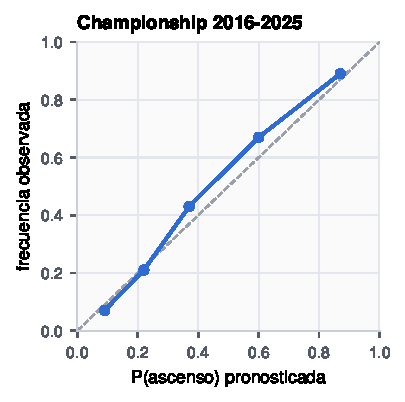
\includegraphics[width=\textwidth]{ascenso}\end{minipage}\hfill
\begin{minipage}{0.56\textwidth}
\caption{Calibración del ascenso en la Championship: probabilidad pronosticada, agrupada en cinco tramos, frente a la frecuencia observada. La suma de probabilidades da 3,0 ascensos por temporada en cada momento.}
\label{fig:ascenso}
\end{minipage}
\end{figure}

El ascenso está calibrado (figura~\ref{fig:ascenso}). El prior propio para los descendidos de la Premier (sección~\ref{sec:champ}) gana $+0{,}0019\pm0{,}0005$ nats por partido ($z=3{,}6$) frente al mismo modelo sin él, $+0{,}0038\pm0{,}0012$ en los partidos de los recién llegados, y mejora el ascenso sobre todo en pretemporada (Brier 0,094 frente a 0,099).

\section{Argentina (R19)}

En 4.218 partidos desde 2016 el modelo de dos latentes gana $+0{,}0035\pm0{,}0019$ ($z=1{,}9$). No alcanza dos errores estándar, pero tampoco hay evidencia de que pierda, así que la regla de la sección~\ref{sec:seleccion} lo deja como oficial. En los 1.944 partidos con cuotas, RPS 0,2134 frente a 0,2140 del núcleo y 0,2071 de Bet365. Con el formato actual hay solo tres torneos para evaluar fuera de muestra (Apertura y Clausura 2025, Apertura 2026). La clasificación a octavos se pronostica bien: Brier 0,12 promediando momentos, frente a 0,25 de repartir 16 cupos entre 30 al azar. Pero los tres campeones fueron sorpresas: Platense, Estudiantes y Belgrano tenían entre 1,4 y 6,3\,\% en todos los momentos, con favoritos de 11 a 23\,\%. Una llave de 16 equipos a partido único con alargue y penales reparte mucho, y tres torneos no alcanzan para evaluar la calibración del campeón.

\section{Una temporada en el sitio}

\begin{figure}[h]
\centering
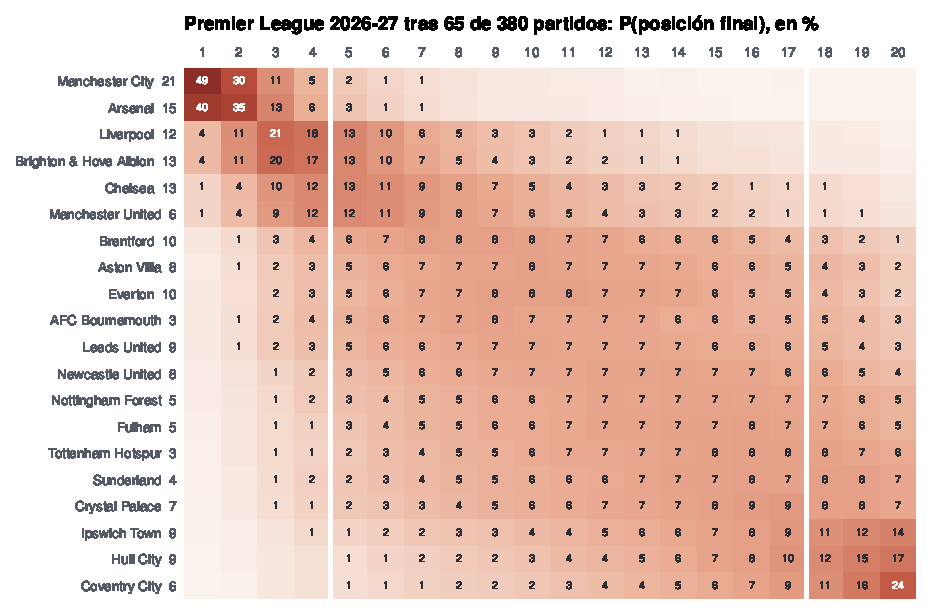
\includegraphics[width=\textwidth]{matriz_premier}
\caption{Matriz de posiciones finales de la Premier League 2026-27 tras 65 de 380 partidos, con 20.000 temporadas simuladas. Junto al nombre, los puntos actuales. Las líneas blancas separan los puestos de Champions y de descenso.}
\label{fig:matriz}
\end{figure}

\begin{figure}[h]
\centering
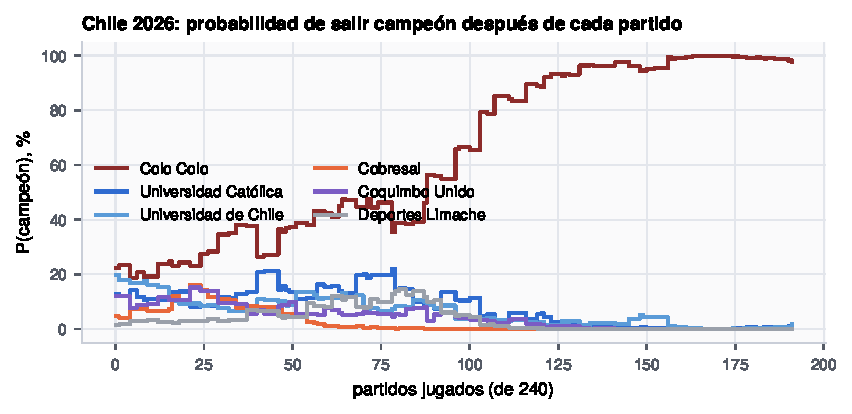
\includegraphics[width=\textwidth]{trayectoria_chile}
\caption{Probabilidad de salir campeón de la Liga de Primera de Chile 2026 después de cada partido, para los seis equipos con más probabilidad en algún momento. Es el gráfico de la ficha de la liga en el sitio.}
\label{fig:trayectoria}
\end{figure}

La figura~\ref{fig:matriz} es la matriz de la Premier a fines de octubre de 2026, y la~\ref{fig:trayectoria} la evolución del campeón de Chile 2026 a lo largo del año. La segunda muestra lo que las matrices estáticas esconden: la probabilidad no se acumula de a poco, sino que cambia a saltos en los partidos que deciden, que son los que la información mutua (sección~\ref{sec:mi}) identifica de antemano.

\section{Competitividad (R11)}
\label{sec:r11}

\begin{figure}[h]
\centering
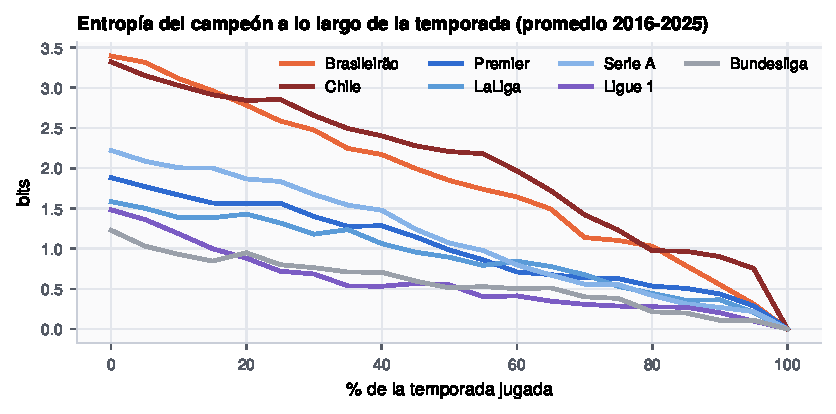
\includegraphics[width=\textwidth]{suspenso}
\caption{Entropía de la distribución del campeón a lo largo de la temporada, promedio de las temporadas 2016-2025 de cada liga.}
\label{fig:suspenso}
\end{figure}

La entropía del campeón en pretemporada separa dos mundos (figura~\ref{fig:suspenso}): Brasil (3,39 bits) y Chile (3,32) empiezan con unos diez candidatos efectivos, y la Bundesliga (1,23) con poco más de dos. La Bundesliga y la Ligue 1 se definen ($P\ge95$\,\%) al 44-46\,\% de la temporada en promedio; Chile y Brasil, al 91-93\,\%. Los campeones más improbables del período, medidos con la probabilidad que tenían en pretemporada, fueron el Lille 2020-21 (1,2\,\%) y el Monaco 2016-17 (1,3\,\%).
